\section{Auswertung}
\label{sec:Auswertung}

% \subsection{a) Detektorscan Gauß-Fit}
\subsection{Detektorscan Gauß-Fit}

\begin{figure}
  \centering
  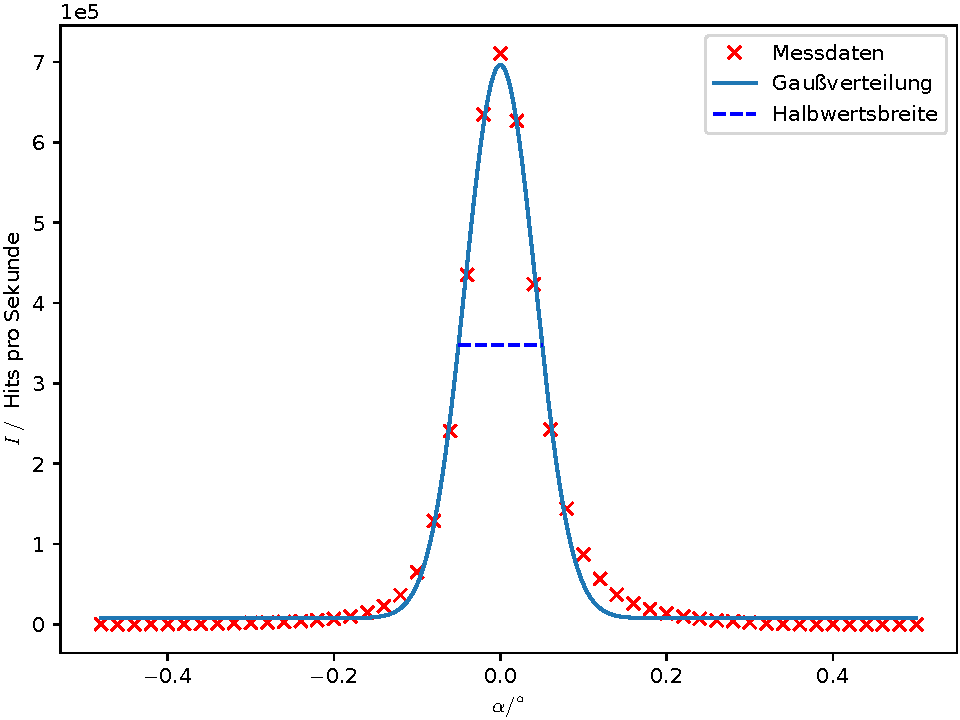
\includegraphics[width=0.7\textwidth]{figures/detectorscan.pdf}
  \caption{Detektorscan mit Gaußfunktion als Ausgleichskurve. Gemessene Inten-
  sität ist gegen den Winkel der Probe zum Detektor aufgetragen.}
  \label{fig:detectorscan}
\end{figure}
\noindent

Der Detectorscan ist in Abb. \ref{fig:detectorscan} dargestellt.
Es wird der Winkel der Probe zum Detektor gegen die gemessene Intensität aufgetragen.
Es wird eine Fit gegen die Gaußfunktion durchgeführt.
\begin{equation}
  I(\alpha) = \frac{a}{\sqrt{2 \cdot \pi \cdot \sigma^2}} \cdot \exp\left(-\frac{(x - \mu)^2}{2 \cdot \sigma^2}\right) + b
\end{equation}

Mithilfe eines Fit werden folgende Parameter bestimmt:

\begin{align*}
  a &= \num{7.29+-0.10e+04} \\
  b &= \num{7.8+-2.1e+03} \\
  \sigma &= \SI{0.0423+-0.0006}{\degree} \\
  \mu &= \SI{-0.0000+-0.0006}{\degree} \, .
\end{align*}

Die Halbwertsbreite $\mathrm{FWHM} = 2\sqrt{2\ln 2}\,\sigma$  und 
maximale Intensität $I_\text{max}$ ergibt sich zu:
\begin{align*}
  \mathrm{FWHM}  &= \SI{0.1003}{\degree} \\
  I_\text{max} &= \num{695956} \, .
\end{align*}



% \subsection{b) Reflektivitätscan}
\subsection{Reflektivitätscan}

\begin{figure}
  \centering
  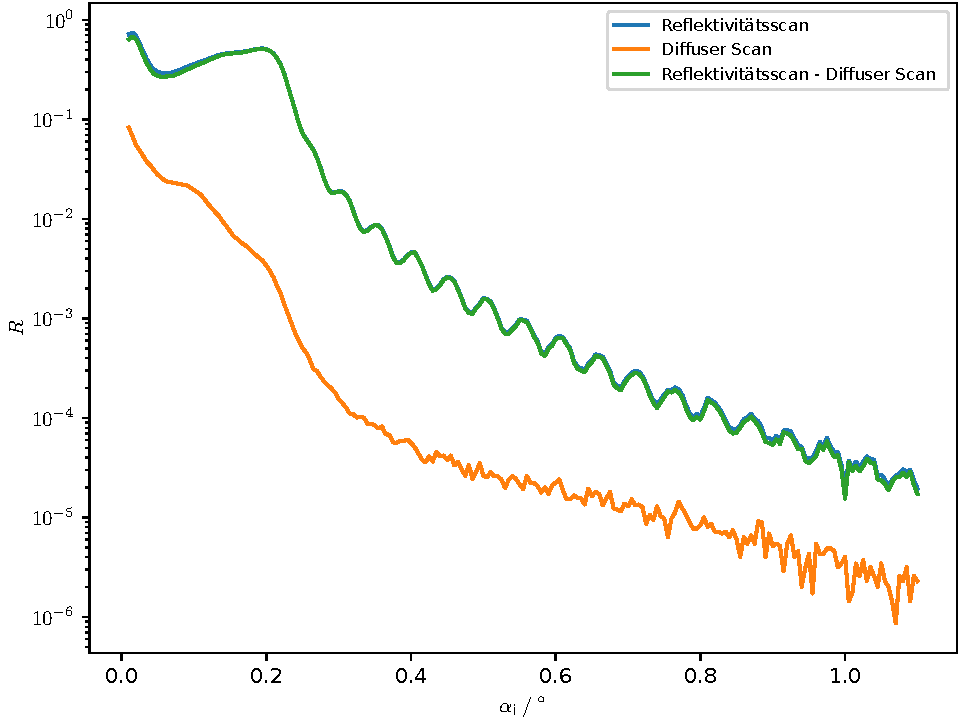
\includegraphics[width=0.7\textwidth]{figures/plot_messung1_diff.pdf}
  \caption{Messdaten des Reflektivitätsscans und diffusen Scans.}
  \label{fig:plot_messung1_diff}
\end{figure}

Die Messung der Reflektivität, des diffusen Scans sowie der Differenz
jener ist in Abb. \ref{fig:plot_messung1_diff} dargestellt.
% messbereich wird eingeschränkt

% \subsection{c) Geometriefaktor}
\subsection{Geometriefaktor}

\begin{figure}
    \centering
    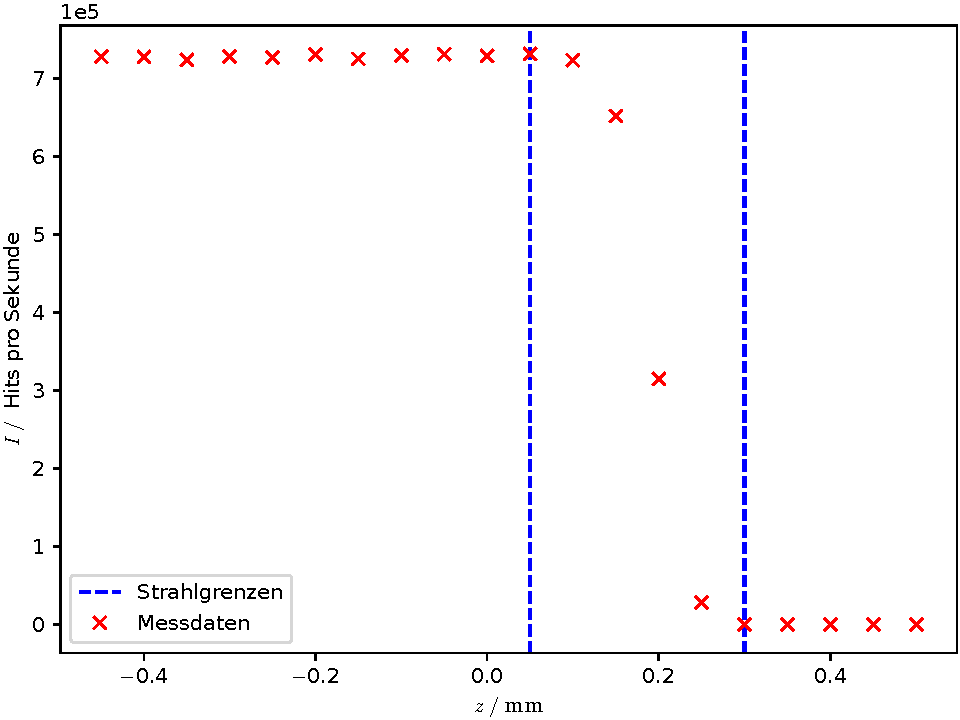
\includegraphics[width=0.7\textwidth]{figures/zscan.pdf}
    \caption{Die Messdaten des Z-scans. Die Schichtdicke ergibt sich zu $d_0=\num{0.25}$.}
    \label{fig:zscanscan}
\end{figure}

\begin{figure}
    \centering
    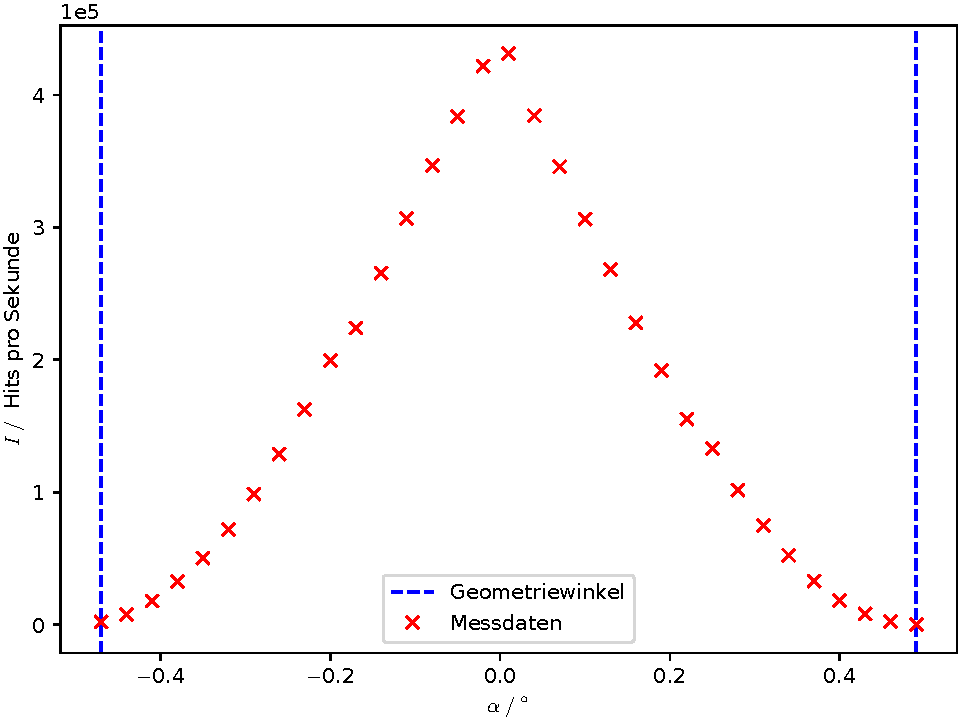
\includegraphics[width=0.7\textwidth]{figures/rockingscan.pdf}
    \caption{Die Messdaten des Rocking-scans. Der abgelesene Geometriewinkel ergibt sich zu $\overline{\alpha_\text{g}} = \SI{0.48}{\degree}$.}
    \label{fig:rockingscan}
\end{figure}
  \noindent

Der Z-Scan sowie Rockingscan mit $\theta = 0$ ist in Abb. \ref{fig:zscanscan} und Abb. \ref{fig:rockingscan}
dargestellt.

Aus dem Rocking-Scan lässt sich der Geometriewinkel ablesen:

\begin{align*}
  \alpha_\text{g,links} &= \SI{0.49}{\degree} \\
  \alpha_\text{g,rechts} &= \SI{-0.47}{\degree} \\
  \overline{\alpha_\text{g}} &= \SI{0.48}{\degree} \, .
\end{align*}

Zur bestimmung des theoretischen Geometriewinkel wird die Strahlbreite $d_0$ am Z-Scan
(Abb. \ref{fig:zscanscan}) abgelesen zu $d_0=\num{0.25}$ und mit der Probenlänge $D = \SI{20}{\milli\meter}$
und Gl. \refeq{eqn:geome} berechnet. Mithilfe des Geometriewinkels werden außerdem die Messdaten 
in Abb. \ref{fig:plot_messung1_diff} korrigiert.

%  \marktodo{vergleich mzwischen eigenem und errechnetem geometriewinkel} 

\begin{equation*}
  \alpha_\text{g,Theorie} = \SI{0.687}{\degree}
\end{equation*}


% \subsection{d) Schichtdicke aus Kissing Oszillationen bestimmen}
\subsection{Schichtdicke aus Kissing Oszillationen bestimmen}

\begin{figure}
  \centering
  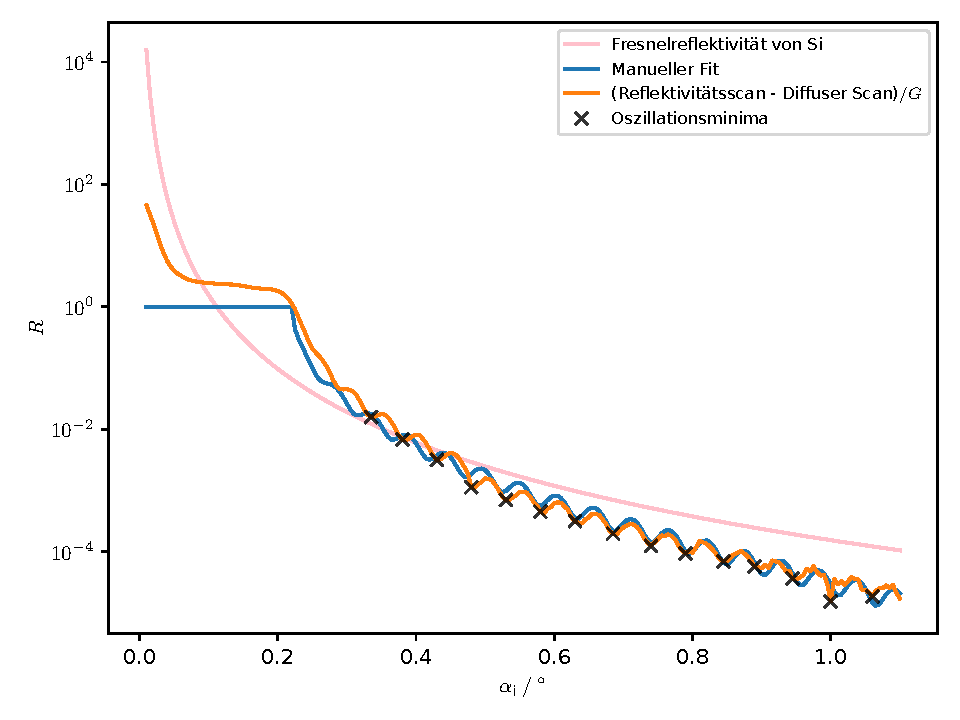
\includegraphics[width=0.7\textwidth]{figures/plot_messung2_parrat.pdf}
  \caption{Ergebnisse der Bestimmung des
  Dispersionsprofils}
  \label{fig:plot_messung2_parrat}
\end{figure}

Nun wird aus den Kiessig Oszillationen die Schichtdicke $d$ bestimmt. 
Es werden die Minima bestimmt und deren Abstände zueinander bestimmt und 
gemittelt ($\overline{\Delta\alpha_\text{i}}$).
Daraus ergibt sich dann über Gl. \eqref{eqn:Kiessig} die Schichtdicke $d_\text{PS}$.

\begin{align*}
  \overline{\Delta\alpha_\text{i}} = \SI{9.04+-0.20e-4}{\,\degree} \\
  d_\text{PS} = \SI{8.52+-0.26e-08}{\meter}
\end{align*}

% \subsection{g) Dispersonsprofil mit dem Parrat-Algorithmus bestimmen und e) Dispersion bestimmen} % parrat 2
\subsection{Dispersonsprofil mit dem Parratt-Algorithmus bestimmen} % parrat 2

In Abb. \ref{fig:plot_messung2_parrat} ist der manuelle Fit mit dem
Parrat-Algorithmus (Gl. \eqref{eqn:parrat_1} abgebildet.
Es wird die Polystyrol (PS) als Schicht 2 und Silizium
(Si) als Substrat bzw. Schicht 3 angenommen.
Die Fresnelkoeffizienten werden mit der RMS–Rauigkeit modifiziert.
Fest angenommen werden die Parameter
 \begin{align*}
  \delta_\text{1,Luft} &= 0 \\
  z_1 &= 0 \\
  \lambda &= \SI{1.54e-10}{\meter}.
\end{align*}

Die Parameter werden so angepasst, dass die berechnete Reflektivität möglichst 
gut mit der gemessenen Reflektivität übereinstimmt.
Für den manuellen Fit in Abbildung \ref{fig:plot_messung2_parrat} werden die folgenden 
Parameter verwendet:
\begin{align*}
  z_2 &= \SI{8.10e-8}{\meter}\\
  \delta_\text{3,Si} &= \num{7.4e-6}\\
  \delta_\text{2,PS} &= \num{1.0e-6}\\
  \sigma_1 &= \SI{6.55e-10}{\meter} \\
  \sigma_2 &= \SI{8.15e-10}{\meter} \\
  \beta_2 &= \num{0.05e-7}\\
  \beta_3 &= \num{0.6e-6}
\end{align*}

%  \marktodo{} 
% Vergleich unserer Schicktdicken (?) Schätzung und den mit dem Parrat Algo ermittelten wert

% \subsection{f) kritischen Winkel bestimmen}
\subsection{kritischen Winkel bestimmen}
Über Gleichung \eqref{eqn:kritschwiknekl} können nun mit den Korrekturen der Brechungsindizes auch die kritischen Winkel der beiden Materialien zu 
\begin{align*}
    \alpha_\text{c,PS} &= \SI{0.081}{\degree} \\
    \alpha_\text{c,Si} &= \SI{0.220}{\degree}
\end{align*}
berechnet werden.

% #  \marktodo{} 
% \subsection{h) Schichtdicken Vergleich}  % parrat 2
% 'Schichtdicke parrat 8.1 e-08



% ????
